\chapter{Implementation}

\section{Python}
\begin{figure}[h]
\centering 
\includegraphics[scale=0.3]{images/python.jpg}
\caption{Python logo}
\end{figure}
\noindent Python is a dynamic language, as in python coding is very easy and 
also it require less coding and about its interpreted nature it is 
just exellent. Python is a high level programming language and Django 
which is a web development framework is written in python language.

Python is an easy to learn, powerful programming language.Python runs 
on Windows, Linux/Unix, Mac OS X. Python is free to use, even for 
commercial products. Python can also be used as an extension language 
for existing modules and applications that need a programmable interface.  
Python is free to use, even for commercial products, because of its 
OSI-approved open source license.
\subsection{Features of Python}
\begin{itemize}
\item Very clear, readable syntax.
\item Strong introspection capabilities.
\item Intuitive object orientation.
\item Natural expression of procedural code.
\item Full modularity, supporting hierarchical packages.
\item Exception-based error handling.
\item Very high level dynamic data types.
\item Extensive standard libraries and third party modules for virtually every task.
\item Extensions and modules easily written in C, C++ (or Java for Jython, or .NET languages for IronPython).
\item Embeddable within applications as a scripting interface.
\end{itemize}
\subsection{Installation of Python}
Installation of python is a very easy proccess.
The current python versions are: Python 2.7.1 and Python 3.2.
Type the commands in the terminal:\\

 \$ wget http://www.python.org/ftp/python/2.7/Python-2.7.tgz\\

 
 \$ tar xzf Python-2.7.tgz\\


This will install the python on your pc/laptop.




\section{Steps of Implementation}
We’re going to employ a Long Short Term Memory (LSTM) model; it’s a particular type of deep learning model that is well suited to time series data (or any data with temporal/spatial/structural order e.g. movies, sentences, etc.).
    \subsection{Data}
    Before we build the model, we need to obtain some data for it. There’s a dataset on Kaggle that details minute by minute Bitcoin prices (plus some other factors) for the last few years (featured on that other blog post). Over this timescale, noise could overwhelm the signal, so we’ll opt for daily prices. The issue here is that we may have not sufficient data (we’ll have hundreds of rows rather than thousands or millions). In deep learning, no model can overcome a severe lack of data. I also don’t want to rely on static files, as that’ll complicate the process of updating the model in the future with new data. Instead, we’ll aim to pull data from websites and APIs.

    \begin{figure}[ht]
        \centering 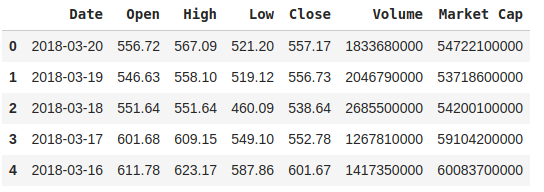
\includegraphics[scale=0.7]{images/data.png}
        \caption{Data used}
    \end{figure}

    As we’ll be combining multiple cryptos in one model, it’s probably a good idea to pull the data from one source. We’ll use coinmarketcap.com. For now, we’ll only consider Bitcoin and Ether, but it wouldn’t be hard to add the latest overhyped altcoin using this approach. Before we import the data, we must load some python packages that will make our lives so much easier.
    
    \subsection{Training}
    We have some data, so now we need to build a model. In deep learning, the data is typically split into training and test sets. The model is built on the training set and subsequently evaluated on the unseen test set. In time series models, we generally train on one period of time and then test on another separate period. 
    As such, the training data may not be representative of the test data, undermining the model’s ability to generalise to unseen data.The most basic model is to set tomorrow’s price equal to today’s price (which we’ll crudely call a lag model). 

    \section{Long Short Term Memory (LSTM)}
    Long short-term memory (LSTM) units (or blocks) are a building unit for layers of a recurrent neural network (RNN). A RNN composed of LSTM units is often called an LSTM network. A common LSTM unit is composed of a cell, an input gate, an output gate and a forget gate. The cell is responsible for "remembering" values over arbitrary time intervals; hence the word "memory" in LSTM. Each of the three gates can be thought of as a "conventional" artificial neuron, as in a multi-layer (or feedforward) neural network: that is, they compute an activation (using an activation function) of a weighted sum. Intuitively, they can be thought as regulators of the flow of values that goes through the connections of the LSTM; hence the denotation "gate". There are connections between these gates and the cell.
    \begin{figure}[ht]
        \centering 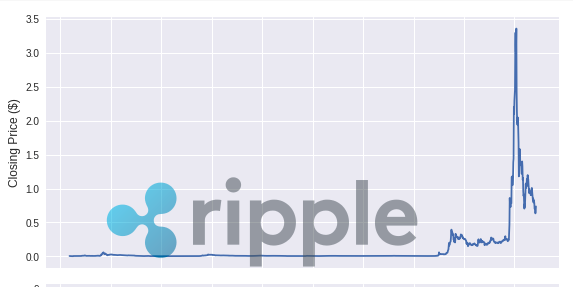
\includegraphics[scale=0.7]{images/lstm.png}
        \caption{Expected Results}
    \end{figure}